\documentclass[12pt]{article}
   
   \usepackage[utf8]{inputenc}
   \usepackage{graphicx}
   \usepackage{float}
   \usepackage{subcaption}
   \usepackage{mathtools}
   \usepackage{amsmath}
   \usepackage{amsfonts}
   \usepackage{multirow}
   \usepackage{multicol}

   \addtolength{\hoffset}{-0.7in}
   \addtolength{\textheight}{1.5in}
   \addtolength{\textwidth}{1.5in}
   \addtolength{\voffset}{-1in}
 
\title{EE 234: Experiment-4\\
Characteristics of Separately Excited DC motor}
       
\author{Group-8 \\Gardas Chaitanya, 180070021  \\
Karthik Gvb, 180070022 \\
Hitesh Kandala, 180070023}
\date{\today}
%_____________________________________________________________________________________________
\begin{document}

  \maketitle
  
    \section{Overview of the Experiment}
        \subsection{Aim}
            To study the variation of speed with
            \begin{itemize}
                \item Armature Voltage
                \item Field current
                and to obtain performance characteristics (T-$\omega$) of a separately excited (S.E.) DC motor.
            \end{itemize}
        \subsection{Methods}
        \begin{figure}[H]
            \centering
            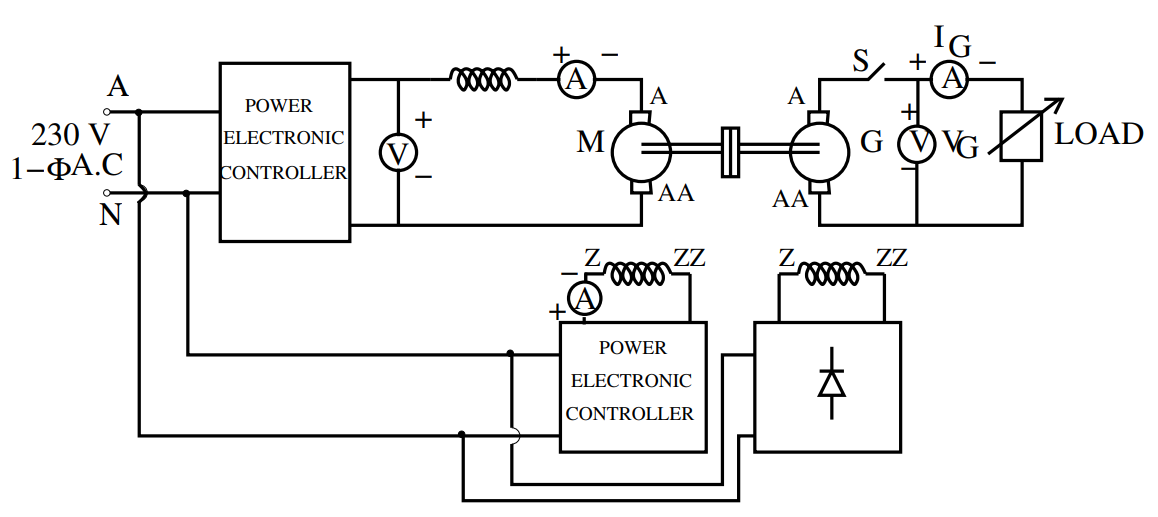
\includegraphics[scale=0.44]{LAB-4/circuit.png}
            \caption{Cicuit for obtaining the speed torque characteristics of the DC motor} % check 9th answer ??
            \label{fig:my_label}
        \end{figure}
        For this experiment we use, the small powered(1.1kW) DC machine as the load and a high powered(1.5kW) machine to obtain the $\omega$ vs T characteristics.
    \clearpage
    \section{Observations}
    In this experiment the load we used for the DC motor is a generator which drives light bulbs. With the efficiency plot($\eta$ vs $P_{out}^g$) of generator and its armature readings($P_{out}=I_a^gV_a^g$) we can obtain input power of generator($P_{in}^g$) which is the output power of the motor(if we assume 100\% coupling efficiency). Knowing the motor speed($\omega$) at that load, we can obtain the torque(T) of the motor at the load, since $P_{out}^m=\omega T$.
    \begin{equation}
        T = \dfrac{V_a^g \times I_a^g}{\eta \omega}
    \end{equation}
    \begin{equation}
        \omega=\dfrac{V_a}{k_e\phi}-\dfrac{R_aT}{(k_e\phi)^2}
    \end{equation}
    
    Slope=$\dfrac{-R_a}{(k_e\phi)^2}$ and y-intercept = \dfrac{V_a}{k_e\phi}.
        \subsection{Armature Voltage Control}
            $I_f$ of DC motor and DC generator were maintained at 0.42A for both the armature voltages
            \begin{table}[H]
                \centering
                \begin{tabular}{|c|c|c|c|c|c|c|c|}
                      %& \multicolumn{2}{c}{DC generator}   \\
                     \hline
                     \hline
                    DC generator & $V_a$(V) & $I_a$(A) & $\omega$(rad/sec) & $P_{out}$(W) & $\eta$ & $P_{in}(W)$ & Torque(N-m)\\
                    \hline
                    \multirow{8}{5em}{Increasing Load} & 164 & 0 & 158.23 & 0 & 0 & 0 & 0\\
                         & 159 & 0.5 & 157.39 & 79.5 & 0.31 & 256.4 & 1.62 \\
                         & 157 & 1.1 & 157.08 & 172.7 & 0.52 & 327.7 & 2.08 \\
                         & 155 & 1.5 & 156.66 & 232.5 & 0.58 & 397.4 & 2.53\\
                         & 152 & 2.1 & 156.13 & 319.2 & 0.65 & 489.5 & 3.13\\
                         & 149 & 2.8 & 155.61 & 417.2 & 0.71 & 585.9 & 3.76\\
                         & 147 & 3.3 & 155.29 & 485.1 & 0.73 & 664.52 & 4.28\\
                         \hline
                         \hline
                \end{tabular}
                \caption{Variation of the speed and output power of the motor with increasing load at $V_a$ = 167V}
                \label{tab:my_label}
            \end{table}
                
            \begin{table}[H]
                \centering
                \begin{tabular}{|c|c|c|c|c|c|c|c|}
                      %& \multicolumn{2}{c}{DC generator}   \\
                     \hline
                     \hline
                    DC generator & $V_a$(V) & $I_a$(A) & $\omega$(rad/sec) & $P_{out}$(W) & $\eta$ & $P_{in}(W)$ & Torque(N-m)\\
                    \hline
                    \multirow{8}{5em}{Increasing Load} & 147 & 0 & 143.25 & 0 & 0 & 0 & 0\\
                        & 144 & 0.5 & 142.52 & 72 & 0.28 & 252.6 & 1.77\\
                        & 141 & 1 & 141.68 & 141 & 0.48 & 290.12 & 2.04\\
                        & 139 & 1.4 & 141.26 & 194.6 & 0.55 & 350 & 2.47\\
                        & 137 & 2 & 140.63 & 274 & 0.62 & 438.4 & 3.11\\
                        & 135 & 2.6 & 140.01 & 351 & 0.67 & 520 & 3.71 \\
                        & 132 & 3.1 & 139.59 & 409.2 & 0.70 & 580.4 & 4.16\\

                         \hline
                         \hline
                \end{tabular}
                \caption{Variation of the speed and output power of the motor with increasing load at $V_a$ = 150V}
                \label{tab:my_label}
            \end{table}
            We ignored power losses for finding the Torque. 
                \begin{figure}[H]
                    \centering
                    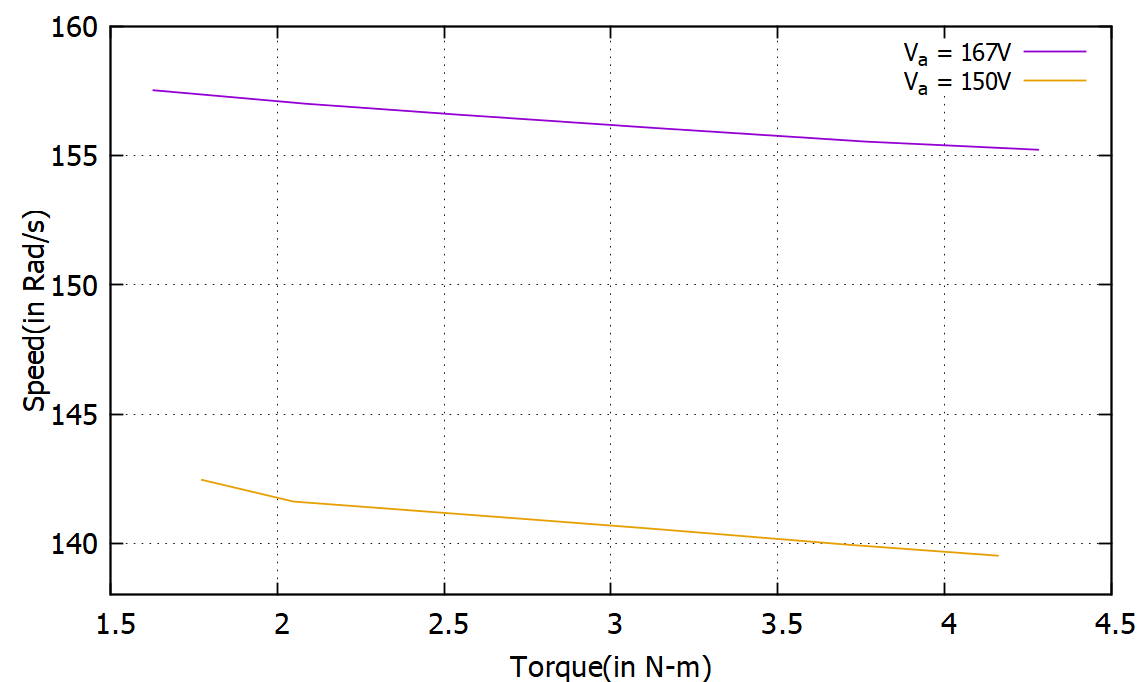
\includegraphics[scale=0.5]{LAB-4/armature.png}
                    \caption{Speed($\omega$) vs Torque characteristics by varying the armature voltage}
                    \label{fig:my_label}
                \end{figure}
        \subsection{Field Weakening}
             $I_f$ of DC generator was maintained at 0.42A for both the field currents and $V_a$ of the DC motor was maintained at 165V
                \begin{table}[H]
                    \centering
                    \begin{tabular}{|c|c|c|c|c|c|c|c|}
                          %& \multicolumn{2}{c}{DC generator}   \\
                         \hline
                         \hline
                        DC generator & $V_a$(V) & $I_a$(A) & $\omega$(rad/sec) & $P_{out}$(W) & $\eta$ & $P_{in}(W)$ & Torque(N-m) \\
                        \hline
                        \multirow{8}{5em}{Increasing Load} & 165 & 0 & 160.32 & 0 & 0 &0&0\\
                                    & 160 & 0.5 & 159.59 & 80 & 0.32 & 250 & 1.56 \\
                                    & 158 & 1.1 & 158.96 & 173.8 & 0.52 & 331.0 & 2.08\\
                                    & 156 & 1.5 & 158.33 & 234 & 0.59 & 396.6 & 2.50\\
                                    & 153 & 2.2 & 157.70 & 336.6 & 0.67 & 502.3 & 3.18\\
                                    & 151 & 2.8 & 157.28 & 422.8 & 0.71 & 595.4 & 3.78\\
                                    & 149 & 3.3 & 156.86 & 491.7 & 0.73 & 668.9 & 4.26\\

                             \hline
                             \hline
                    \end{tabular}
                    \caption{Variation of the speed and output power of the motor with increasing load at $I_f$ = 0.4A}
                    \label{tab:my_label}
                \end{table}
                
                \begin{table}[H]
                    \centering
                    \begin{tabular}{|c|c|c|c|c|c|c|c|}
                          %& \multicolumn{2}{c}{DC generator}   \\
                         \hline
                         \hline
                        DC generator & $V_a$(V) & $I_a$(A) & $\omega$(rad/sec) & $P_{out}$(W) & $\eta$ & $P_{in}(W)$ & Torque(N-m) \\
                        \hline
                        \multirow{8}{5em}{Increasing Load} & 168 & 0 & 163.36 & 0 & 0 & 0 & 0\\
                                & 164 & 0.5 & 162.42 & 82 & 0.32 & 256.2 & 1.57\\
                                & 161 & 1.1 & 161.79 & 177.1 & 0.53 & 334.1 & 2.06 \\
                                & 159 & 1.5 & 161.37 & 238.5 & 0.59 & 404.2 & 2.50\\
                                & 156 & 2.2 & 160.84 & 343.2 & 0.67 & 512.2 & 3.18\\
                                & 154 & 2.8 & 160.42 & 431.2 & 0.71 & 603.0 & 3.76\\
                                & 152 & 3.4 & 160.32 & 516.8 & 0.74 & 692.7 & 4.32\\
                             \hline
                             \hline
                    \end{tabular}
                    \caption{Variation of the speed and output power of the motor with increasing load at $I_f$ = 0.37A}
                    \label{tab:my_label}
                \end{table}
                \begin{figure}[H]
                    \centering    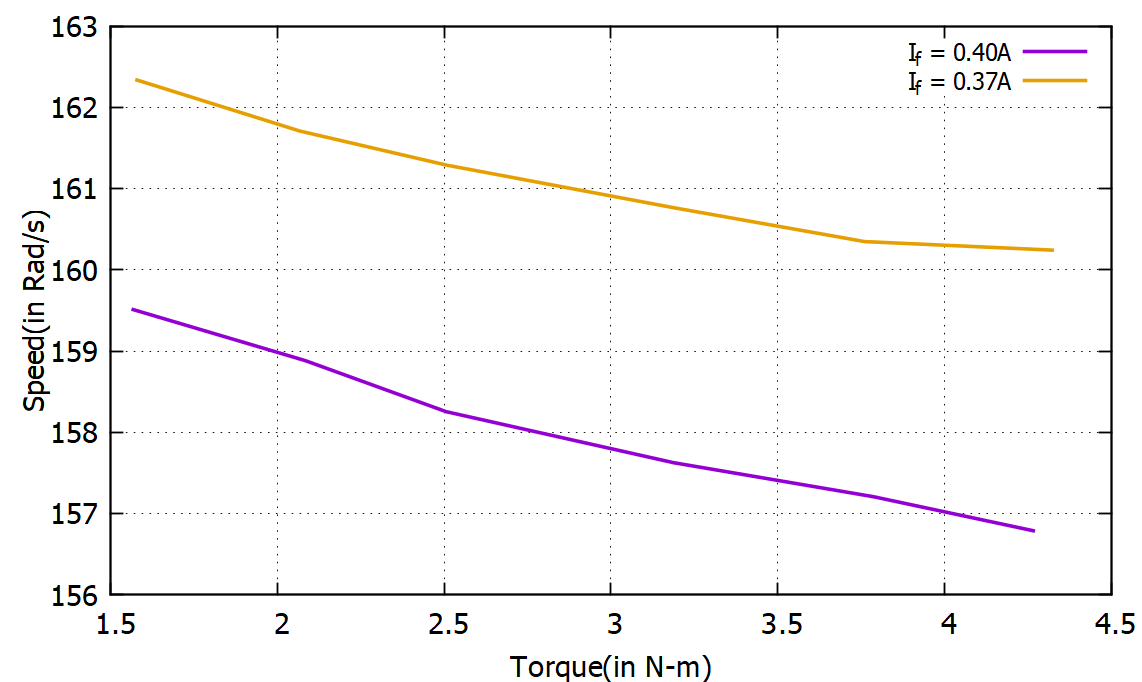
\includegraphics[scale=0.5]{LAB-4/field.png}
                    \caption{Speed($\omega$) vs Torque characteristics by varying the field voltage}
                    \label{fig:my_label}
                \end{figure}
    \section{Conclusion}
    Hence from the armature voltage control and field varying methods we observe that the $\omega$-T characteristics are in accordance with the Eqn.1 and are linear.
    
    In armature voltage control method, the value of the intercept decreased as we decrease the armature voltage, with slope remaining unchanged.
    
    While in the field voltage varying method, as we decrease the field the slope of the increased and showing a similar trend in the intercept values.
    \section{Questions to be answered}
    1. The condition to develop steady torque is that the relative speed between the two fields (in this case $F_s$ and $F_a$.) should be zero. In other words, the two fields should be stationary w.r.t cach other. In dc motor, the speed of $F_s$ is zero (stator coil is stationary and it is excited by dc current), while the armature is rotating. Explain how is the above condition satisfied?\vspace{0.1cm} \\
    \textbf{Ans}: If the DC motor has only one coil then the field produced by it would be rotating but in reality there are many coils i.e a winding and are displaced angularly such that all the coils can be viewed as if they are not moving, they all interchange their places. So the total armature field produced is stationary and is quadrature to the stator field.     
    \vspace{0.2cm}\\
    2. Explain why the full field and reduced armature voltage is applied to dc motor while starting.\vspace{0.1cm} \\
    \textbf{Ans}: At starting induced emf($E_b$) is zero($\omega = 0$), So applying high (rated) voltage generates huge current in the armature coils and severely damages the components of motor. Also we want to increase $\omega$ as soon as possible to increase $E_b$ and then armature voltage can be increased, which can be achieved by applying full stator field (T $\propto \phi$ ).
    \vspace{0.2cm}\\
    3. Whether the speed is independent of the direction of rotation? If it isn't what could be the reason?\vspace{0.1cm} \\
    \textbf{Ans}:The speed is dependent on the direction of rotation, as in reversed direction either the stator field is reversed or the armature field is reversed($T = K_e\phi I_a$) and if the flux (either armature or stator) is keep on applied in a particular direction then the iron core magnetizes to a particular direction, which results to residual flux in the core. Hence on reversing the direction of rotation, speed decreases as the effective flux is less than the expected.    
    \vspace{0.2cm}\\
    4. Armature reaction improves the speed regulation' Is this statement true? Justify your answer.\vspace{0.1cm} \\
    \textbf{Ans}:Yes, Armature reaction improves the speed regulation. Armature reaction is effect of armature flux on the characteristics of the DC motor, armature flux distorts the field flux which results to reduction in the overall flux. This is nothing but the field weakening which increases $\omega$. So on increasing load torque flux decreases to counteract the reduction in $\omega$, similarly when load torque is reduced armature reaction decreases increasing the effective flux thereby regulating the speed of the motor.   
    \vspace{0.2cm}\\
    5. What may happen if the field circuit gets open circuited during motoring?\vspace{0.1cm} \\
    \textbf{Ans}: If the field circuit gets open circuited during motoring then field flux drops to residual flux which is very small. At that instant $E_b$ reduces leading to large flow of current in the armature coil($\omega \text{ doesn't change immediately}$) which thereby damages the machine.
    \vspace{0.2cm}\\
    6. Which type of motor is most suitable for electric traction?\vspace{0.1cm} \\
    \textbf{Ans}: DC series motor is most suitable for electric traction systems because traction systems require high starting torque which is available with DC series motors as torque is proportional to the square of the current, at zero speed there is no back-emf therefore the current is limited only by resistance, so the current and torque are high.
    \vspace{0.2cm}\\
    7. What are the limitations of S.E. dc motor?\vspace{0.1cm} \\
    \textbf{Ans}: It is not suitable for traction type of loads, two power supplies are required, starting the motor is not very fast. Works on DC supply whereas the available power supplies are in AC. 
    \vspace{0.2cm}\\
    8. Why is it mentioned in section-2.1.2 that the maximum speed of operation is about 150\% of the rated speed?\vspace{0.1cm} \\
    \textbf{Ans}: Rated speed is the speed at rated armature voltage, rated armature current and rated field voltage, speed can be increased by decreasing stator field ( field weakening) hence the maximum speed operation is higher than rated speed.  
    \vspace{0.2cm}\\
    9. In dc series motor the field winding is connected in series with the armature. Can a separately excited motor be converted to series motor by connecting the field in series? Justify your answer.\vspace{0.1cm} \\
    \textbf{Ans}: No, a separately excited motor can't be converted to series motor by just connecting the field in series. 
    The field winding of shunt motors are designed to hold small currents. But using it in series, would require a high current than their rated value to pass through to get the rated torque. Hence the performance of the motor decreases.
    \vspace{0.2cm}
            
  
\end{document}